\documentclass[tikz]{standalone}
\usepackage{tikz}
\usetikzlibrary{arrows.meta, calc, positioning, quotes}
\usepackage{amsmath}
\usepackage{amssymb}
\usepackage{bm}

\begin{document}
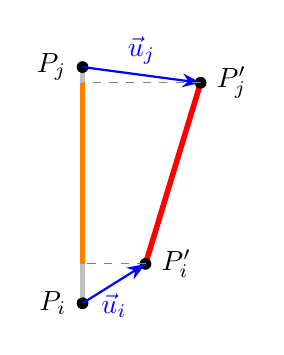
\begin{tikzpicture}[
    dot/.style={circle, fill, inner sep=1.5pt},
    vec/.style={-Stealth, thick},
    projection/.style={dashed, gray}
]

% Definiere Koordinaten
\coordinate (Pi) at (0, 0);
\coordinate (Pj) at (0, 3);

\coordinate (ui) at (0.8, 0.5);
\coordinate (uj) at (1.5, -0.2);

\coordinate (Pi_prime) at ($(Pi) + (ui)$);
\coordinate (Pj_prime) at ($(Pj) + (uj)$);

% Zeichne ursprünglichen Stab
\draw[line width=2pt, lightgray] (Pi) -- (Pj);
\node[dot, label=left:$P_i$] at (Pi) {};
\node[dot, label=left:$P_j$] at (Pj) {};

% Zeichne verschobenen Stab
\draw[line width=2pt, red] (Pi_prime) -- (Pj_prime);
\node[dot, label=right:$P'_i$] at (Pi_prime) {};
\node[dot, label=right:$P'_j$] at (Pj_prime) {};

% Zeichne Verschiebungsvektoren
\draw[vec, blue] (Pi) -- (Pi_prime) node[midway, below] {$\vec{u}_i$};
\draw[vec, blue] (Pj) -- (Pj_prime) node[midway, above] {$\vec{u}_j$};

% Zeichne relativen Verschiebungsvektor
\coordinate (delta_u_start) at ($(Pi) + (2,3)$);

% Projektion
\draw[line width=2pt, orange] ($(Pi)!(Pj_prime)!(Pj)$) -- ($(Pi)!(Pi_prime)!(Pj)$);
\draw[projection] (Pj_prime) -- ($(Pi)!(Pj_prime)!(Pj)$);
\draw[projection] (Pi_prime) -- ($(Pi)!(Pi_prime)!(Pj)$);

\end{tikzpicture}
\end{document}
